\documentclass[12pt]{article}
\usepackage{graphics}
\usepackage[top=1in,bottom=1in,left=1in,right=1in]{geometry}
\usepackage{alltt}
\usepackage{array}	
\usepackage{graphicx}
\usepackage{tabularx}
\usepackage{verbatim}
\usepackage{setspace}
\usepackage{listings}

\usepackage{amssymb,amsmath, amsthm}
\usepackage{zed-csp}
\usepackage[cc]{titlepic}

\title{COMP 335: Introduction to Theoretical Computer Science\\
\ \\
Assignment 3}
\author{Nathan Grenier}
\date{\today \\ Fall 2024}

\begin{document}
\begin{spacing}{1.5}
      \maketitle

      \newpage

      \begin{enumerate}

            \item[1.] [20 Points] For each of the following languages over $\Sigma = \{a,b\}$, write a regular grammar and then convert it into an equivalent NFA using the procedure described in class.

                  \begin{enumerate}
                        \item[(a)] (10 Points) $L(r) \text{ where } r= ((a+b)(a+b))^*b+a((a+b)(a+b))^*$

                              \textbf{G:}
                              \begin{itemize}
                                    \item $S \rightarrow A|B|\lambda$
                                    \item $A \rightarrow aD|bD$
                                    \item $D \rightarrow aD|bD|bS$
                                    \item $B \rightarrow aC$
                                    \item $C \rightarrow aaS|abS|baS|bbS|$
                              \end{itemize}

                              \textbf{Equivalent NFA of G:}

                              \begin{figure}[h!]
                                    \centering
                                    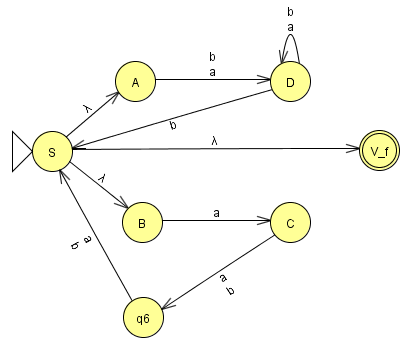
\includegraphics[width=0.65\textwidth]{img/q1/q1a(NFA).png}
                              \end{figure}
                              \newpage
                        \item[(b)] (10 Points) $\{w \in \{a,b\}^* : w \text{ ends in $a$ and $|w| \equiv 1$ } (\mod 3) \}$

                              \textbf{G:}
                              \begin{itemize}
                                    \item $S \rightarrow aA|bA|a$
                                    \item $A \rightarrow aB|bB$
                                    \item $B \rightarrow aS|bS$
                              \end{itemize}

                              \textbf{Equivalent NFA of G:}

                              \begin{figure}[h!]
                                    \centering
                                    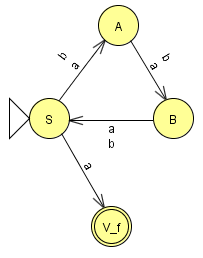
\includegraphics[width=0.35\textwidth]{img/q1/q1b(NFA).png}
                              \end{figure}

                  \end{enumerate}

                  \newpage
            \item[2.] [25 Points] Fix an alphabet $\Sigma$. For any string $w$ with $|w| \geq 2$, let $skip(w)$ be the string obtained by removing the first two symbols of $w$. Define 2 operators on languages:
                  $$f_1(L)=\{w \in \Sigma^* : skip(w) \in L \}$$
                  $$f_2(L)=\{skip(w) \in \Sigma^* : w \in L \}$$

                  \begin{enumerate}
                        \item[(a)] (5 Points) Consider $L' = L(bba^*)$ over tha alphabet $\Sigma = \{a,b \}$. Write a regular expression representing $f_1(L')$. Write another regular expression representing $f_2(L')$.
                              $$r_1 = (a+b)(a+b)bba^*$$
                              $$r_2 = a^*$$

                        \item[(b)] (10 Points) Claim: For every regular language $L$ the language $f_1(L)$ is regular. Clearly state whether the claim is TRUE or FALSE, and then prove your answer.

                              \textbf{Answer:} TRUE

                              \textbf{Proof:}

                        \item[(c)] (10 Points) Claim: For every regular language $L$ the language $f_2(L)$ is regular. Clearly state whether the claim is TRUE or FALSE, and then prove your answer.

                              \textbf{Answer:} FALSE

                              \textbf{Proof:}
                  \end{enumerate}

                  \newpage
            \item[3.] [20 Points] For each of the following languages, use the Pumping Lemma and/or closure properties of regular languages to show that the language is not regular.

                  \begin{enumerate}
                        \item[(a)] (10 Points) $L_1=\{0^k1^l : k \geq l^4 \geq 0\}$

                        \item[(b)] (10 Points) $L_2=\{a^n : n \text{ is not a perfect cube}\}$
                  \end{enumerate}

      \end{enumerate}

\end{spacing}

\end{document}